\newpage

\section*{ $^{115}$In(n,$\gamma$)$^{116}$In }

Power Level: 100 kW(th) \\
Time at Power: 30.0 s \\
Wait Time:  2.0 h \\
Counting Time: 60.0 s \\
Total Activity at Removal: 1.64e+03 $\mu Ci$

\begin{table*}[h]
\centering
\begin{tabular}{ |c|c|c|c|c|c| }
 \hline
 Position & Mass $mg$ & Counting Activity $\mu Ci$ & Area (Counts) & Error \% \\
 \hline 
 1 & 1.10 & 7.28e+01 & 2.12e+06 & 0.0687 \\ 
\hline
 2 & 1.10 & 1.17e+02 & 3.42e+06 & 0.0541 \\ 
\hline
 3 & 1.10 & 1.05e+02 & 3.05e+06 & 0.0573 \\ 
\hline
 4 & 1.10 & 5.29e+01 & 1.54e+06 & 0.0805 \\ 
\hline
\end{tabular}
\end{table*}

\begin{figure}[h]
\centering
\begin{subfigure}{.5\textwidth}
  \centering
     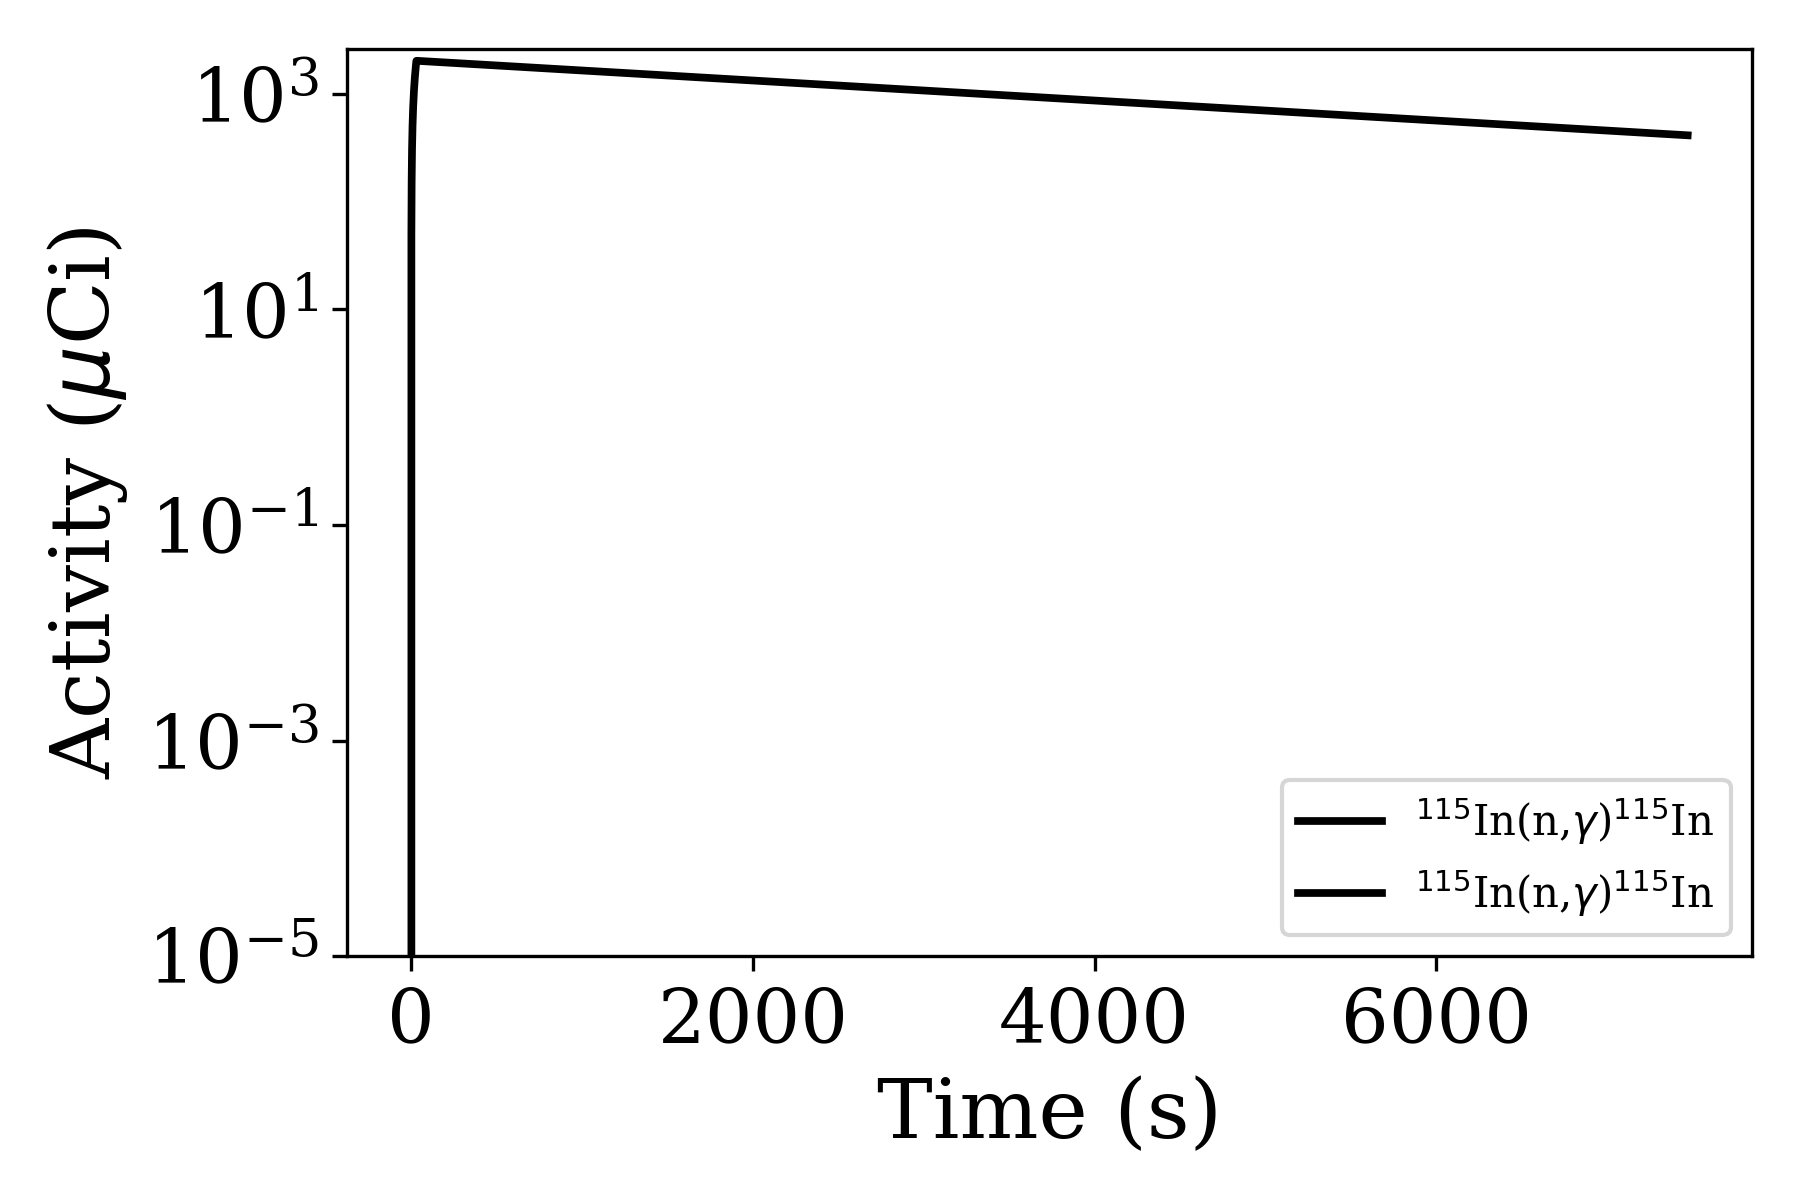
\includegraphics[width=.8\textwidth]{plot/In-115(n,gamma)In-116_wisconsin1} 

  \caption{Activity}
\end{subfigure}%
\begin{subfigure}{.5\textwidth}
  \centering
     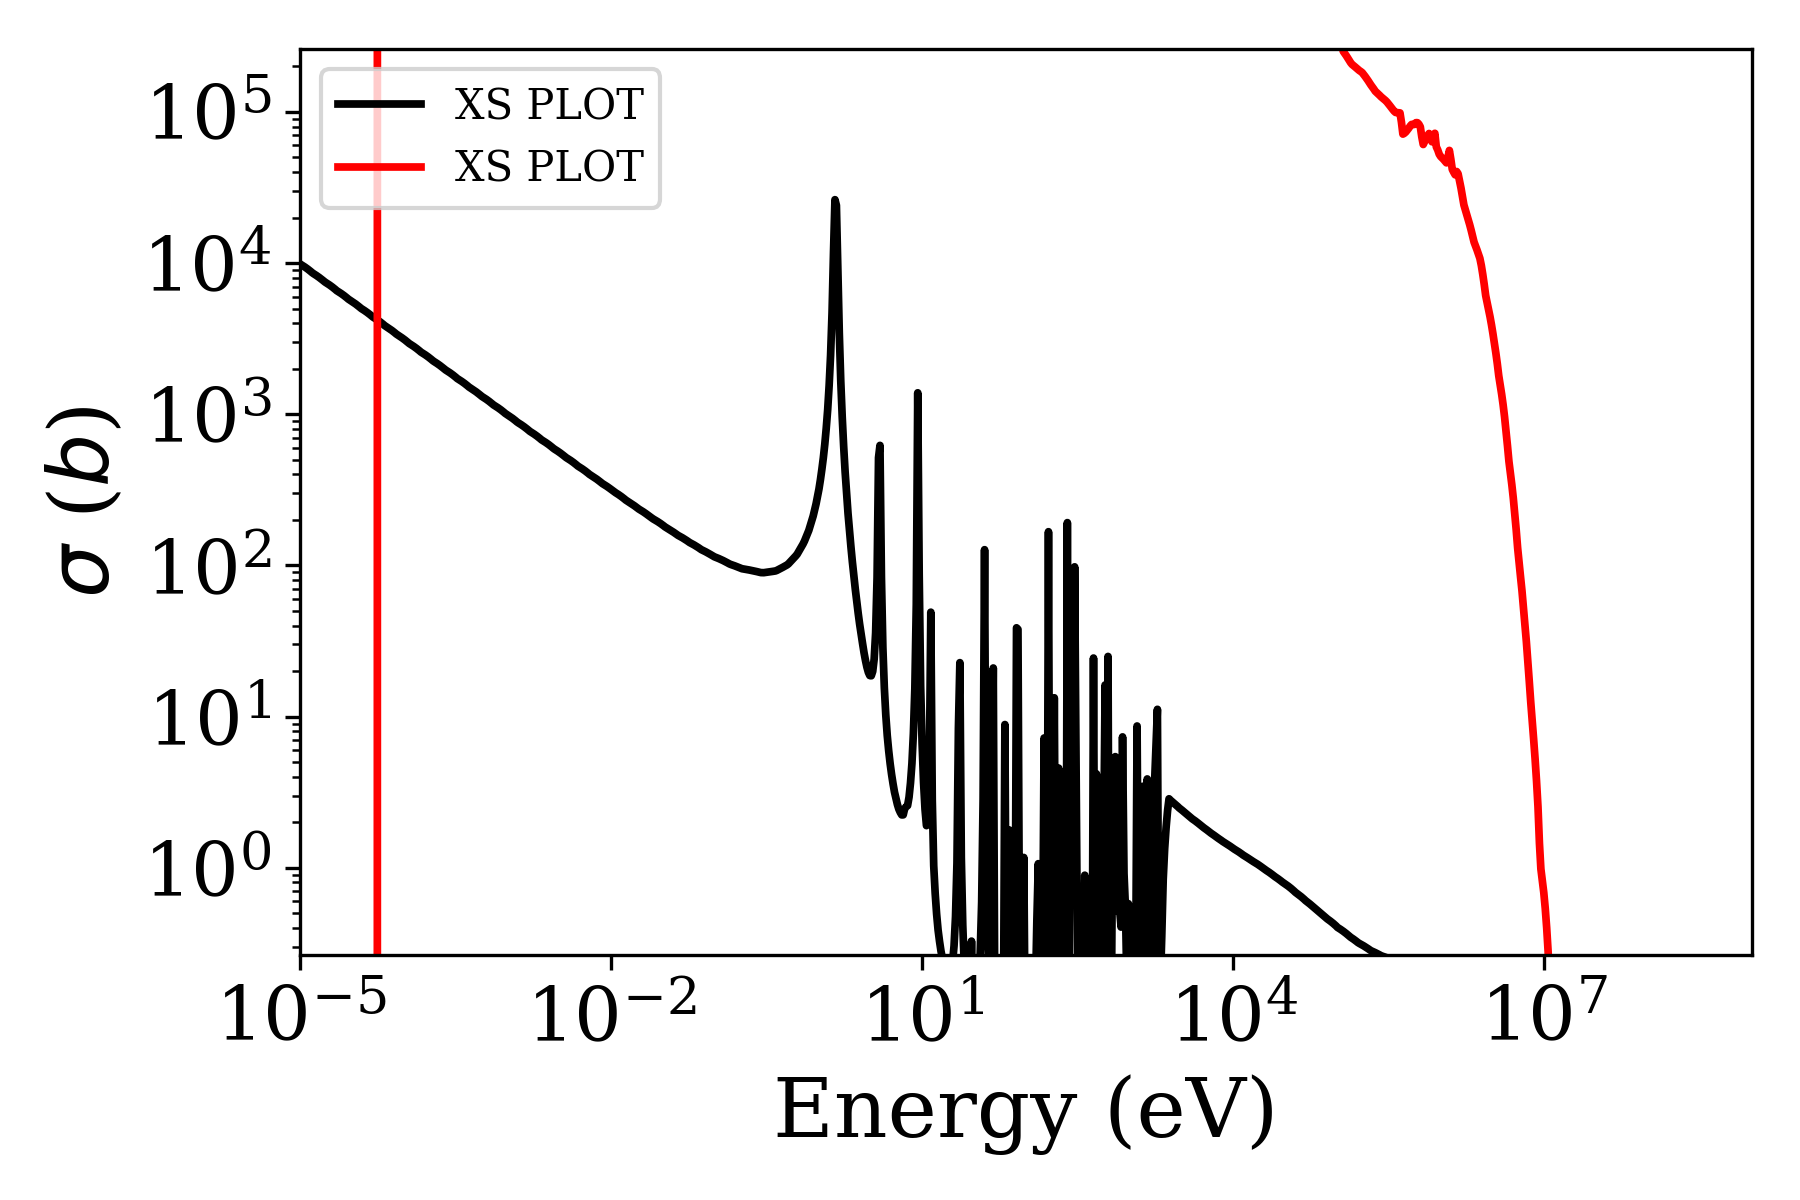
\includegraphics[width=.8\textwidth]{plot/In-115(n,gamma)In-116} 

  \caption{Cross Section}
\end{subfigure}
\end{figure}

\begin{table*}[h]
\centering
\begin{tabular}{ |c|c|c|c|c|c|c| }
 \hline
 Reaction & T$_{1/2}$ & ROI (eV) & Important Gammas (keV) \\
 \hline 
 $^{115}$In(n,$\gamma$)$^{116}$In & 54.0 m & 1.41e-02, 1.63e+00 & 1293(0.8) \\ 
\hline
\end{tabular}
\end{table*}
